\section{Ground Systems}
\label{sec:gndsys}
\subsection{Launch Pad} %Johnny

For the launch pad, the newly constructed Space Team launch pad will be used. It is large enough to fit all ground system components and with a new rail extension the now \SI{7}{\meter} launch rail is long enough to allow the rocket to take off at a decent speed. Since it is already built, it saves time and resources which would be required to construct a new one, specific to \uH. \cref{fig:gro_lp} shows the launch pad in usage.

\begin{figure}[H]
    \centering
    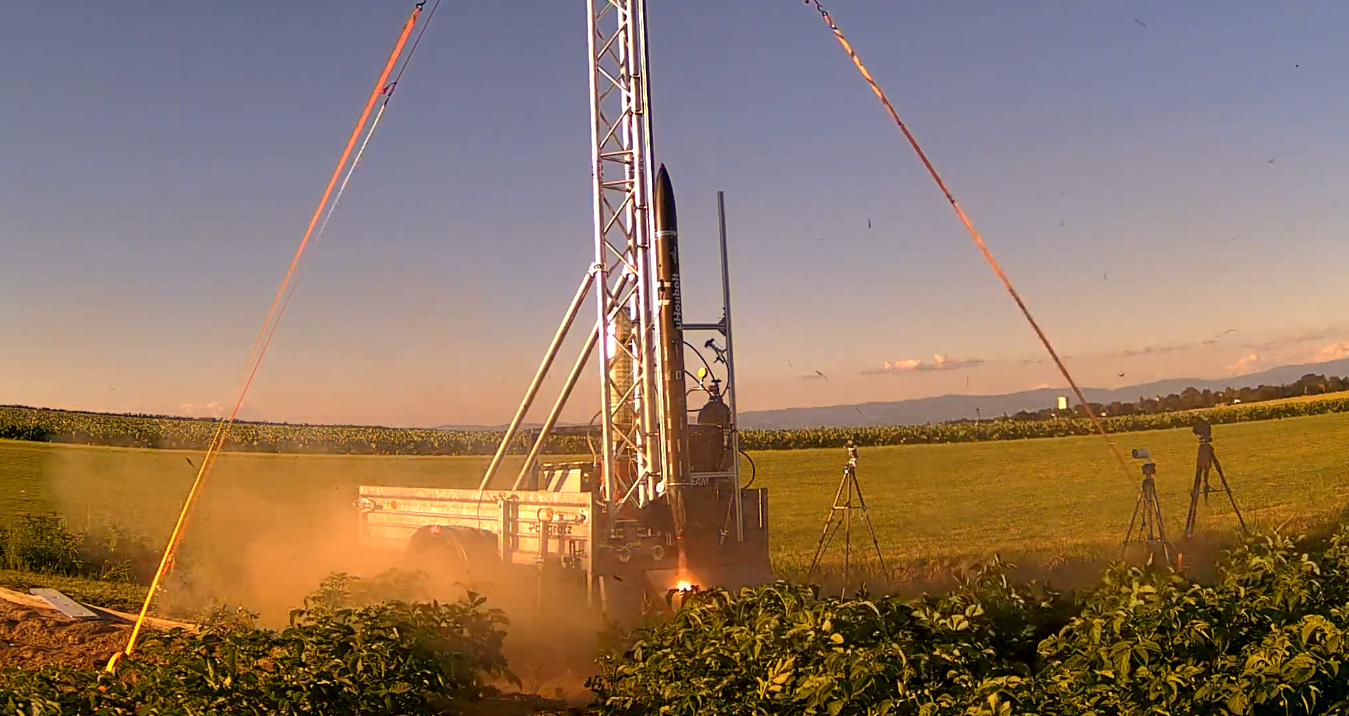
\includegraphics[width = \textwidth]{GroundSystems/uhb_on_rail.png}
    \caption{Launch Pad with \uH during lift-off on first test flight}
    \label{fig:gro_lp}
\end{figure}

\subsubsection{Rail}
The launch rail consists of pieces of 30x\SI{30}{\milli\meter} aluminium extrusion profile, each mounted to one corner of a section of triangular aluminium truss. Pipe clamps screwed into one side of the profiles are used to connect the profile to the truss sections. The whole rail consists of  three truss sections, two of them measuring \SI{2.5}{\meter}, one at \SI{2}{\meter}, which are connected by slotting the ends of one section into the ends of the previous section and securing them with cross bolts. The extrusion profiles on top are then aligned using long sliding blocks in the lateral grooves, resulting in a seven meter long continuous launch rail. The rail buttons on the rocket ride in the dorsal groove.
One of the truss sections is mounted to the launch pad trailer using hinges. This allows the lowest rail section to be folded down during transport. For a launch the other two rail sections are added and the whole rail, once in the upright position, is braced against the trailer as well as guyed to the ground. See \cref{fig:gro_lp}.

\subsubsection{Holddown} \label{sec:holddown}
While the rocket will be guided along the rail using rail buttons its vertical movement will be restricted by an additional holddown system. Two bars are placed on the top and bottom of the lower rail button. The top bar is connected to a pivoting mechanism, while the bottom bar is connected to a plate with a force measurement system. By measuring the weight of the rocket while tanking the fill level of the oxidizer tank can be estimated. During the ignition sequence, the upper bar of the holddown system prevents a premature liftoff. As soon as the chamber pressure (and thus the thrust) is high enough, the system unlocks the pivoting mechanism with a COTS RC servo motor and releases the rocket. This ensures that a liftoff can only happen when the engine performs as expected and accelerates the vehicle to a velocity sufficient for aerodynamic stability when leaving the launch rail. It also offers an additional abort scenario in case of a loss of control over the fuel or oxidizer valves by constraining the rocket to the launch rail for the entire burn duration.

\subsection{Tanking Infrastructure}

The tanking infrastructure (containing oxidizer and pressurant loading system) is mounted on the trailer next to the launch rail. It contains all the necessary plumbing and electronics to remotely tank oxidizer and pressurant and disconnect the umbilicals before the launch.

\begin{figure}[h]
    \centering
    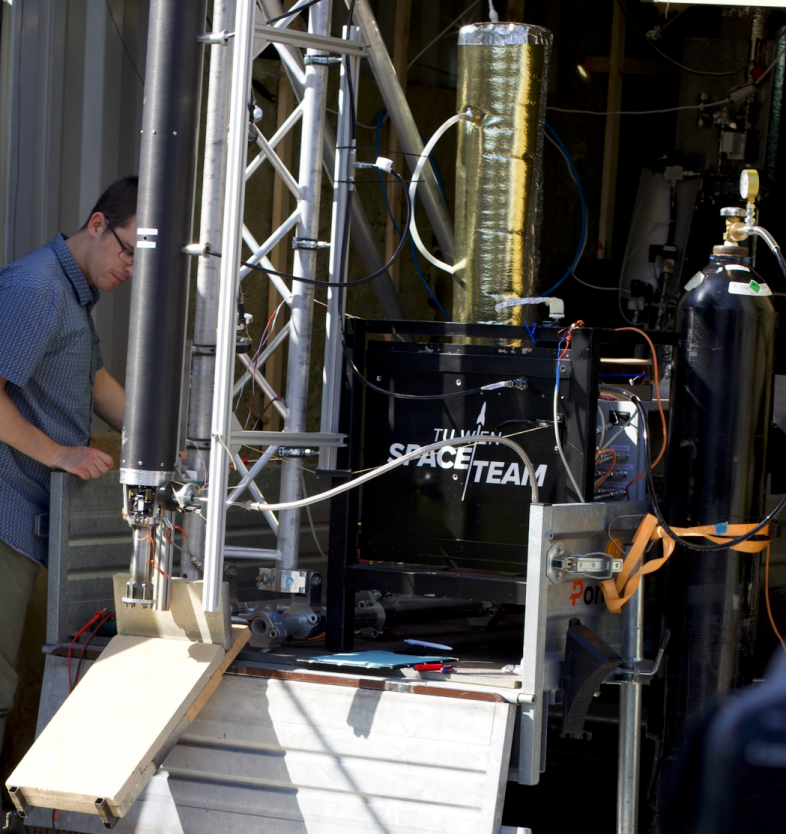
\includegraphics[width=0.5\textwidth]{GroundSystems/gse_uhoubolt.png}
    \caption{Rocket on rail (left) and oxidizer \& pressurant loading system (right)}
    \label{fig:gse_umbilicals}
\end{figure}

\subsection{Oxidizer Loading System}
\label{sec:groundsys_oxload}

See \cref{sec:sysarch_prop_oxLoad} from the Propulsion chapter for a more complete description of the process. This chapter mostly focuses on the physical setup. For a piping diagram see \cref{fig:full_pnid}.

Nitrous Oxide is supplied from a standard gas cylinder which is mounted upside down in the propellant loading system. A heat exchanger jacket is placed over the cylinder in order to be able to control its temperature. In cooling mode the jacket is supplied with water slightly above \SI{0}{\celsius}, while in heating mode the water has \SI{30}{\celsius}.
The hot and cold water is stored in two insulated tanks on the back of the propellant loading system.

This heat exchanger jacket mostly consists of a modified PVC drainage pipe.
To install the gas cylinder the bottom flange of the heat exchanger jacket is placed upside down on the bottle neck, with the valve sticking through a hole in the flange and secured using a nut which fits the threads normally used for the bottle cap. The cylinder is then turned on its head and the bottom flange inserted into a cradle on the propellant loading cart where it is secured using cross pins. Then the jacket is installed and fastened to the bottom flange using three toggle latches around its outside. Lastly the cooling/heating system is connected to the heat exchanger using two hoses equipped with quick-connect fittings. The feed line enters the heat exchanger on the bottom while the return line exits it on the top.

At this point the nitrous oxide cylinder can be connected to the oxidiser loading system and the oxidiser and pressurant umbilicals can be connected to the rocket. Before the start of actual oxidizer loading the tank inside the rocket needs to be pre-pressurized with nitrogen which uses the same pressurization system as the final pressurization before launch via the pressurization umbilicals.

After completion of the filling process (indicated by liquid being vented through the solenoid valve instead of gas), the fill valve is closed. Opening a vent valve in the oxidiser loading system depressurizes the umbilical in preparation for its remote controlled detachment. This is needed as the quick disconnect fittings in use for the umbilicals can't be remotely disconnected under pressure. The entire oxidizer loading process starting from opening the fill valve to the oxidizer tank being full takes about one minute.

The pressurant fill system then supplies nitrogen from a standard \SI{300}{\bar} cylinder to the two pressurant tanks in the vehicle. Same as the oxidizer loading system it also uses two valves for filling and umbilical venting, but it does not need a temperature management system.

%This is achieved by holding the N2O bottle at a temperature of at least \SI{10}{\celsius}. The tank in the rocket will be colder than this, because some of the nitrous oxide already in the rocket will be bled off to reduce the temperature, using the same effect as is tried to counteract in the source tank with the heating.

%It is imperative to not increase the temperature too much, because nitrous oxide goes critical at \SI{36.5}{\celsius} which encourages the spread of decomposition processes (due to e.g. impurities) of the nitrous oxide which is a big safety risk.

The individual steps that need to be executed during the filling procedure are listed in section \ref{sec:oxidizer_loading}.

\subsubsection{Temperature Control}
Switching between the heating and cooling cycle is facilitated by actuating two 3-way valves, one in the feed line, one in the return line and only turning on the hot or cold water feed pump.

The water in the heating cycle is brought to temperature using a \SI{3}{\kilo\watt} water heater controlled by a temperature sensor inside the hot water reservoir, while the cooling cycle temperature is maintained by periodically dumping dry ice into the cold water reservoir. Although water ice can also be used if dry ice is not available, using dry ice is the preferred option, since it doesn't influence the water level in the system.

\subsubsection{Electronics Components}

\begin{figure}
    \centering
    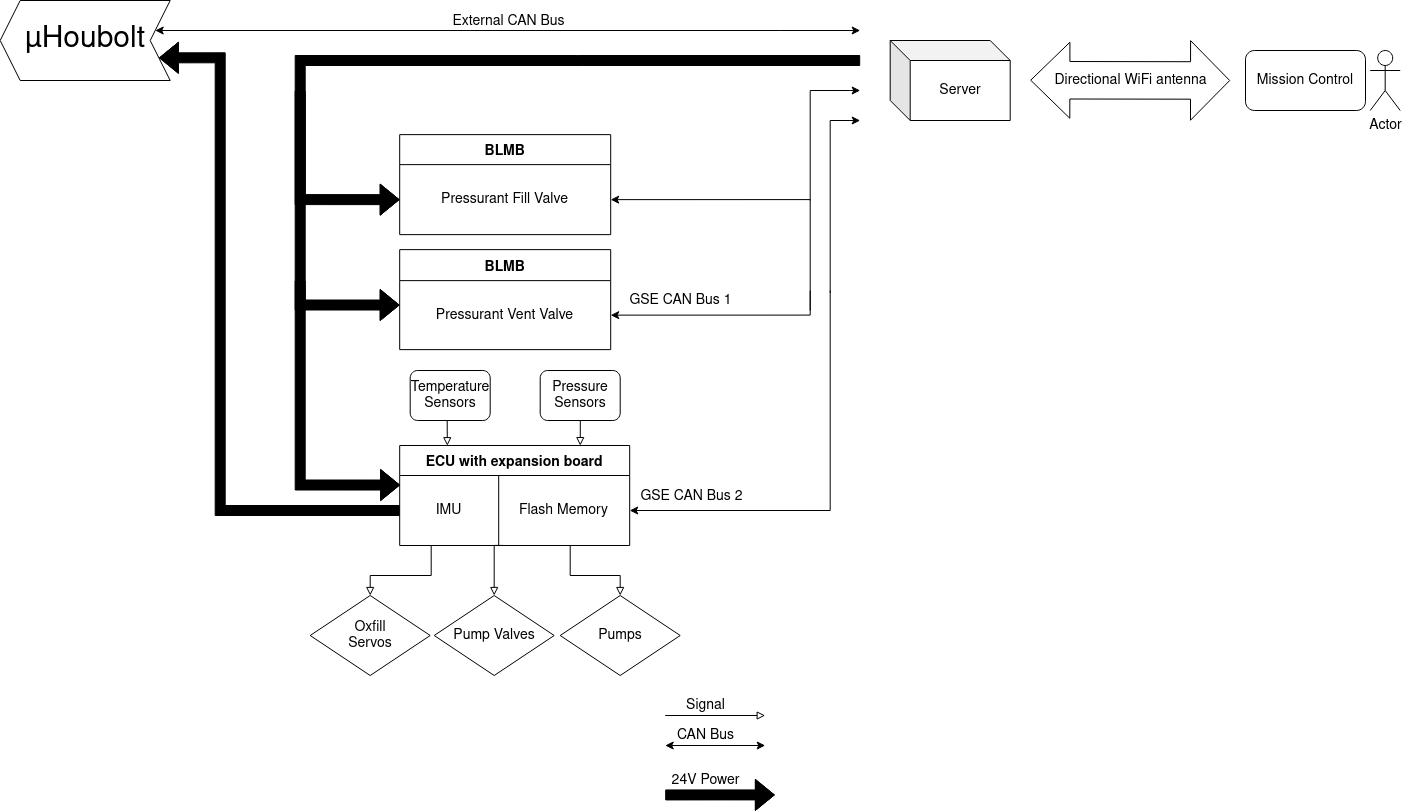
\includegraphics[width=0.9\textwidth]{GroundSystems/GSE_Blockdiagram.png}
    \caption{Subsystem Block Diagram, see \cref{fig:avi_ssbd} for the block diagram for the Avionics.}
    \label{fig:gse_ssbd}
\end{figure}

The Ground Support Equipment, including the oxidizer loading system uses a modified version of our Engine Control Unit PCB, with the outputs for the igniter being repurposed for driving the water pumps through relays. The nitrogen pressurization also takes care of the oxidizer tank pre-pressurization and utilizes two SRAD Turboservos which replaced COTS servo motors as those couldn't provide a high enough torque for actuating the valves at such high pressures, which also have their accompanying BLMB (Brushless Motor Board) PCB connected. All of these components are connected via CAN to Mission Control.

The Turboservos are SRAD servo motors which utilize a brushless DC motor connected to a servo gearbox and a rotary encoder. The control PCB is connected directly to the CAN bus and takes position commands which it translates into movement for the motor to reach the desired position which is then checked in a control loop with the rotary encoder.

The water temperature is being measured with two submersible NTC Resistors which can measure the temperature accurate to +/-\SI{0.5}{\percent}.


\subsection{Pressurant Loading System} %Johnny
%P\&ID
%Safety Analysis, Eignungsnachweis kritischer Komponenten\\ \\

\subsubsection{Overview}
The pressurant tanks inside the rocket, which are actually paintball tanks rated for \SI{310}{\bar} are pressurised to \SI{300}{\bar} through two seperate umbilicals which are fed from a nitrogen gas cylinder, as can be seen in \cref{fig:full_pnid}. Since the target pressure in the rocket's tanks is the same as the pressure inside the full nitrogen cylinder a pressure regulator is not required. Pressurisation of the rocket as well as depressurisation of the oxidiser loading system can be remotely controlled using two motorised valves.

\subsection{Umbilicals} %Johnny
\label{sec:umbilicals}

\subsubsection{Electric Connection}
The electrical umbilical is magnetically connected to a port at the top of the vehicle. During lift-off the electrical umbilical will automatically disconnect as the rocket moves along the launch rail.

\subsubsection{Fluid Umbilicals}
The fluid umbilicals are connected at three points along the side of the rocket. The upper two supply the pressurant gas while the lower one provides the oxidiser. Thus the two pressurant umbilicals consist of flexible high pressure gas line that is able to withstand the \SI{300}{\bar} inside the pressurant system. The oxidiser umbilical is a piece of flexible tubing compatible with nitrous oxide, which is reinforced with metal braiding along the outside. All three fluid umbilicals terminate in quick-disconnectors that have their counterparts on the rocket. The ends of the umbilicals are connected to the strongback that is pulled away from the rocket before the launch. In order to not apply any unnecessary torque to the rocket that could damage the rail or the railbuttons umbilical disconnectors (see \cref{fig:umbilical_disc}) are used to separate the lines from the rocket.
They are spring loaded devices that are placed over the quick-disconnects. When the strongback is pulled back it first pulls a pin (uper left) out of the umbilical disconnector that releases the spring, which presses against the airframe using a pusher plate (black). A lip at the front of the tube engages with the quick-disconnect and releases it. The strongback, which is connected to the umbilical and disconnector through the line in the lower left then pulls the device away from the rocket.

In order for this system to work reliably the oxidiser and pressurant lines first have to be depressurised.

\begin{figure}
    \centering
    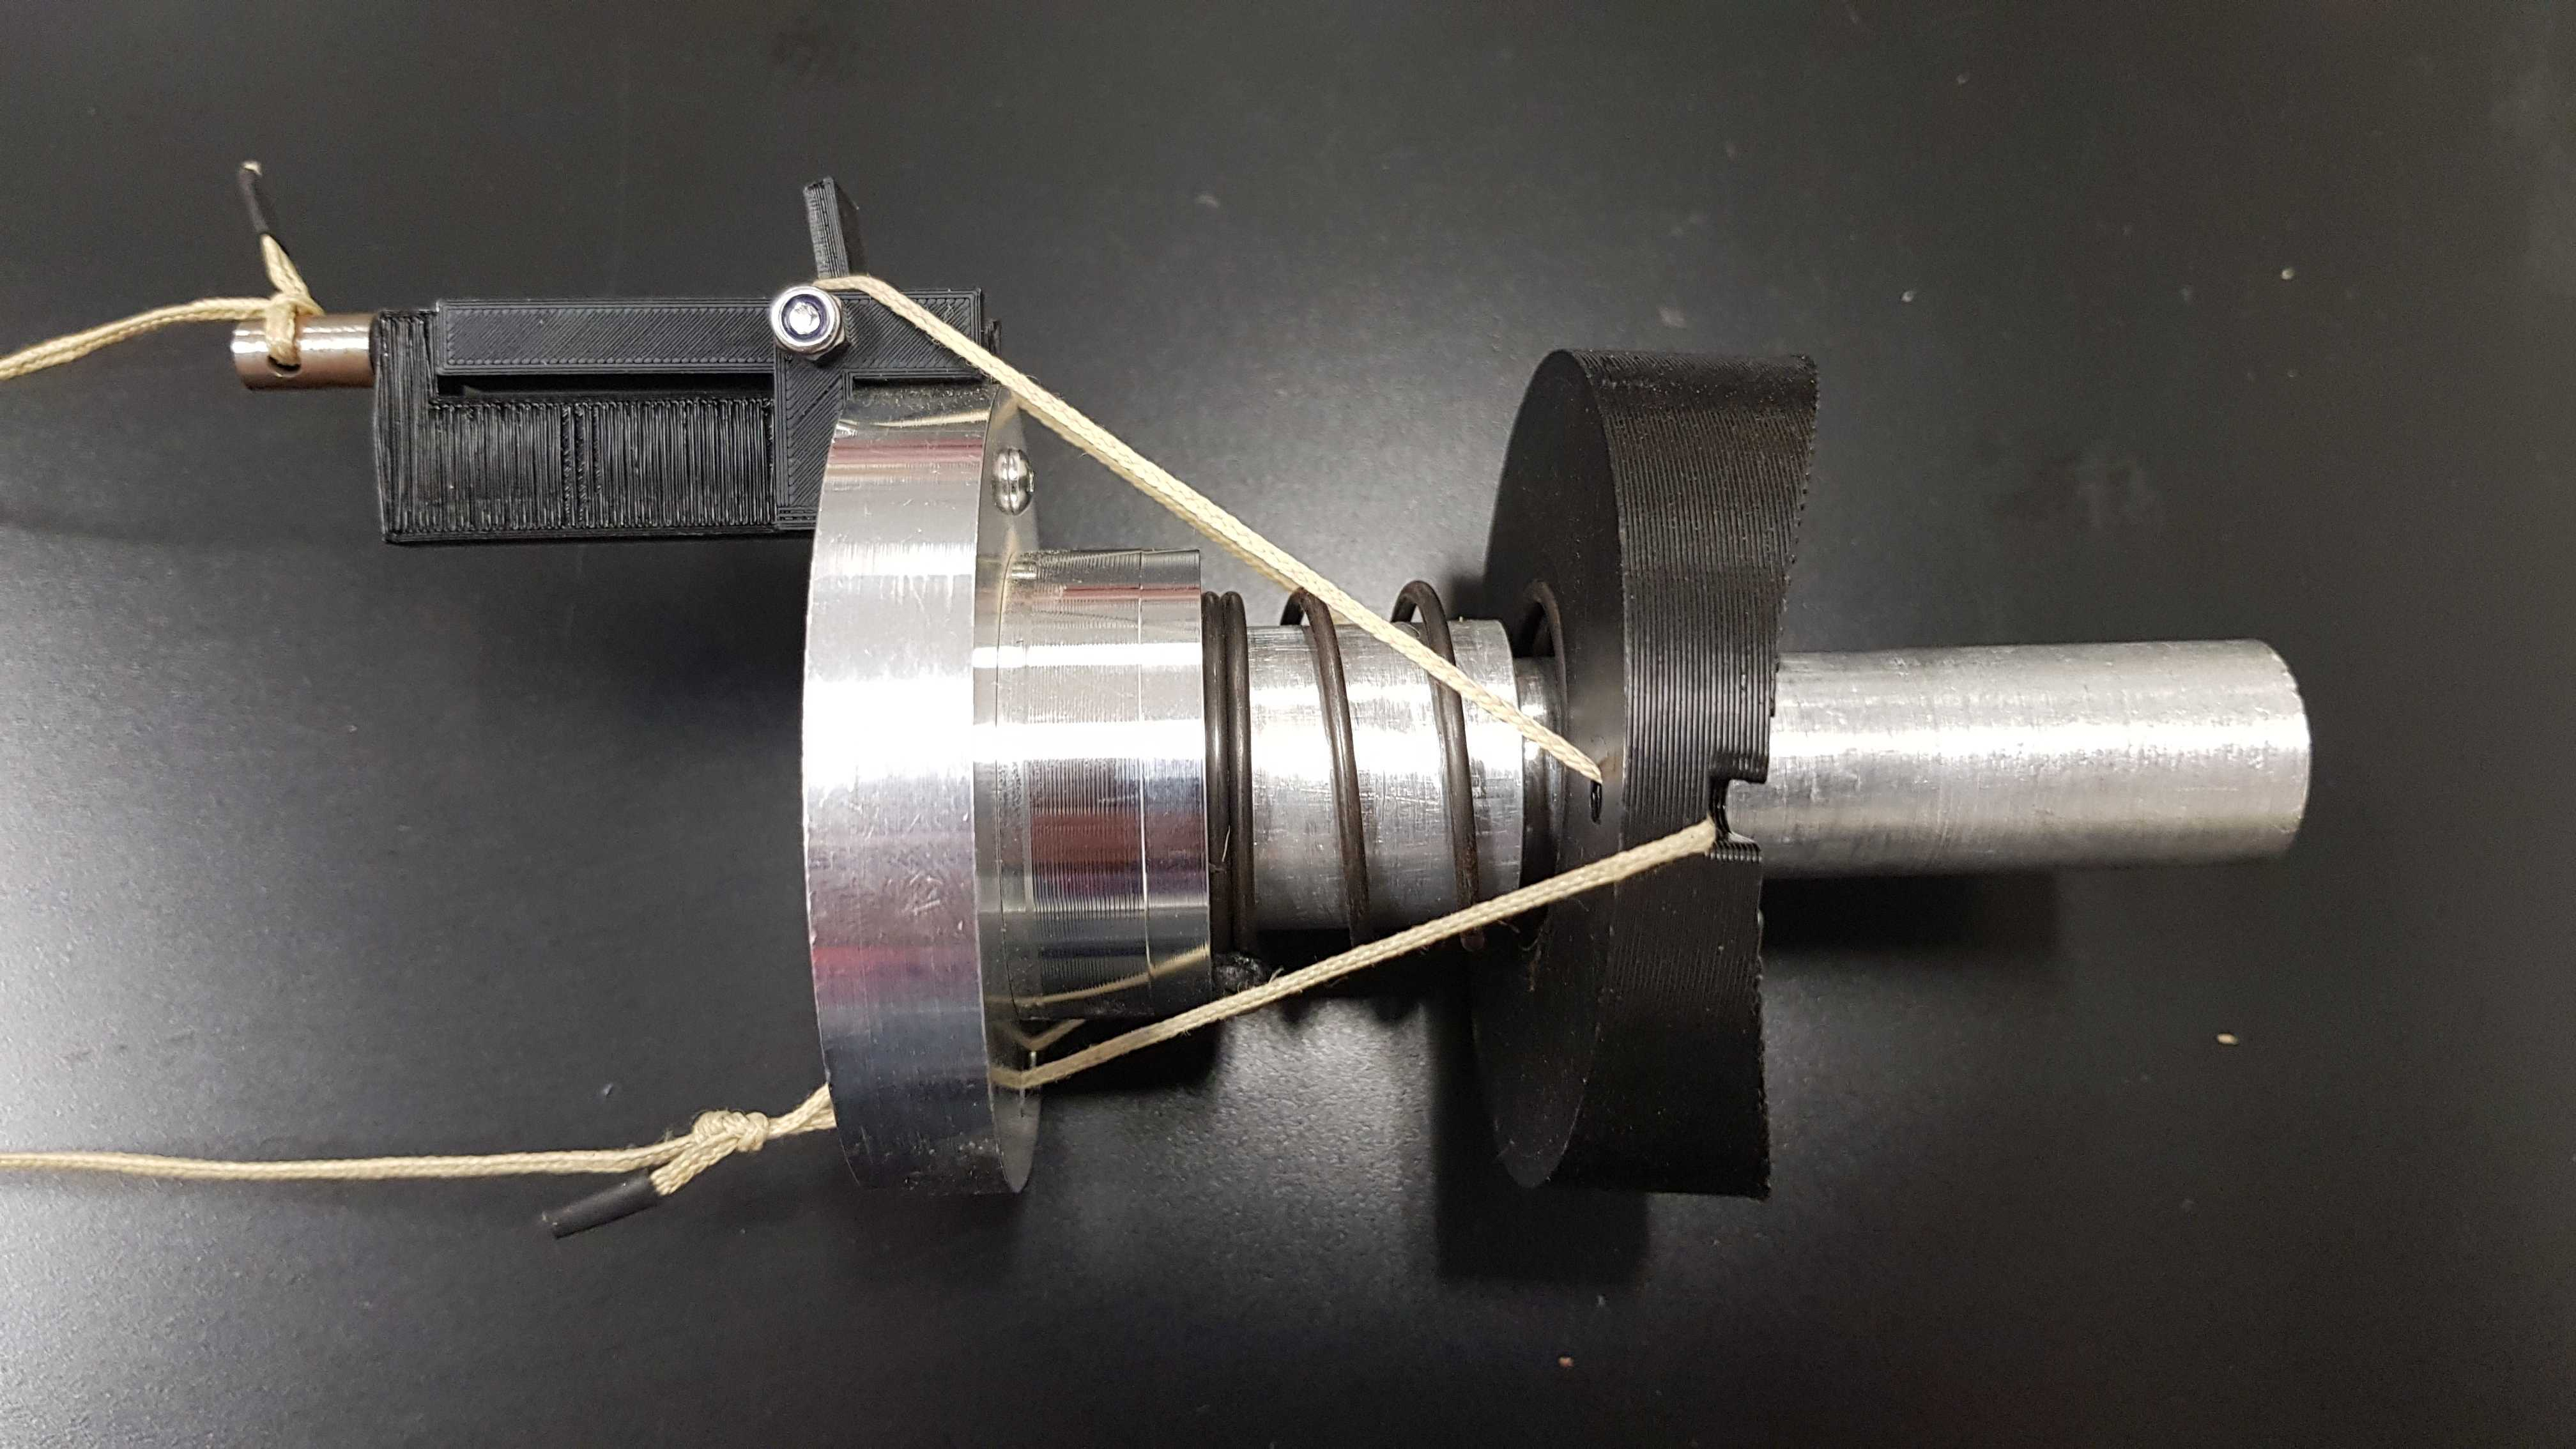
\includegraphics[width=0.9\textwidth]{GroundSystems/Umbilical_Disconnect.jpg}
    \caption{Umbilical Disconnector}
    \label{fig:umbilical_disc}
\end{figure}

\subsection{Ground Support Equipment Electronics}

This section has overlap with information on the Mission Control Software, so if interactions are unclear it is advised to read \cref{sec:software} from the appendices which covers the the software architecture.

Similarly to the rocket itself, the electronics in the launch pad are connected to the main Ubuntu Server via CAN Bus and is controlled via the same Low Level Server and Mission Control data flow as the rocket. There are three components in the GSE: A modified ECU (Engine Control Unit) board whose igniter outputs are wired to the cooling and heating pump of the oxidizer loading system, and two BLMB (Brushless Motor Board).

The launch pad is wired to the Ubuntu Server in a mobile rack with a CAN cable and the server rack is connected to the Mission Control with a directed radio link. In the server rack, connected directly to the server via LAN, a Raspberry Pi single board computer with a LoRa shield is used for the \SI{433}{\mega\hertz} radio connection to the rocket during flight.

The entire GSE is powered using mobile power generators and during launch preparations the electronics umbilical also provides power to the rocket, keeping the internal batteries charged until automatic disconnect at lift-off.